\section{Motivation}

Personal, academic, and industrial motivations drive this thesis. 

This research is conducted in collaboration with \textit{Epidemic Sound AB (ES)} \cite{EpidemicSite}, a prominent Swedish company that provides a global library of over 40,000+ royalty-free soundtrack music and 90,000+ sound effects, and the \textit{Music Technology Group (MTG)} at Universitat Pompeu Fabra in Barcelona, Spain. 

The MTG specializes in developing new technologies related to sound and music, including music information retrieval, digital signal processing, computational models of music perception and cognition, and interactive music systems. 

The collaboration with Epidemic Sound and the MTG aims to deepen our understanding of music and its fundamental structures, potentially leading to advancements and benefits for the company's technical products, services, and MIR academic research.

\subsubsection{Personal motivation}

As a music enthusiast, professional musician, and scholar, I am passionately committed to exploring the foundational elements of musical composition, investigating the diverse techniques employed in creating musical works, and deciphering the intricate relationships among them. This passion fuels my quest for knowledge on extracting valuable information embedded within music in any domain, being my main interest in the audio and symbolic domain, contributing to developing more sophisticated and effective music-related technologies and solutions in the industrial landscape.

I advocate for exposure as the primary method of learning music, emphasizing the importance of immersing oneself in various musical experiences to foster a holistic understanding of music as an art form. Individuals can cultivate well-rounded musical expertise by engaging with different styles, genres, techniques, and learning approaches, ultimately promoting creativity and experimentation.

\subsubsection{Academic motivation}

The emergence of self-supervised models that learn embedding spaces for retrieving musical content from audio signals has unveiled new opportunities in academic research. By capturing high-level semantic information from raw audio data in an unsupervised manner, these models can potentially revolutionize various aspects of the music industry. Their applications encompass music information retrieval, sharing learned latent representations for MIR \cite{HamelTransferSimilarity}, and fostering interdisciplinary research and innovation in musicology, computer science, and artificial intelligence.

\subsubsection{Industrial and corporate motivation}

In the industrial and corporate realm, the embedding spaces generated by these models can be utilized to create personalized and intelligent music recommendation systems \cite{Chen2020LearningRecommendation}\cite{epidemic}, facilitate effective enforcement of intellectual property rights, and contribute to the development of more sophisticated audio editing-production tools and technical products \cite{WonEmotionStories}. These advancements ultimately enhance our interaction with music in the digital age, promoting innovation and collaboration across the music industry.

While it is true that the theoretical foundations of machine learning can be traced back to the pioneering work of figures such as Alan Turing and Claude Shannon in the mid-twentieth century, we are currently experiencing a period of significant breakthroughs in AI research \cite{Vaswani2017AttentionNeed}. These breakthroughs have facilitated the implementation of AI in widely used products \cite{OpenAI2023GPT-4Report}. Many researchers and corporations are keen to stay abreast of these developments and contribute to this exciting and rapidly evolving field.

\subsection{About music aural skills and high-level perceptual concepts}

I have consistently been inspired by musicians and researchers who strive to uncover musical ground truth within an existing tonal paradigm, such as Heinrich Schenker and his school of thought, or by challenging it, exemplified by Arnold Schoenberg or George Russell \cite{LydianRussell}. These approaches aim to identify abstract concepts that reinforce or disrupt the tonal foundation. Their ultimate goal is to advance the tonal landscape, providing musicians with a dependable playground for growth, development, and further understanding of tonal paradigms.

%%%%%%%%%%%%%%%%%%

\begin{figure}[ht]
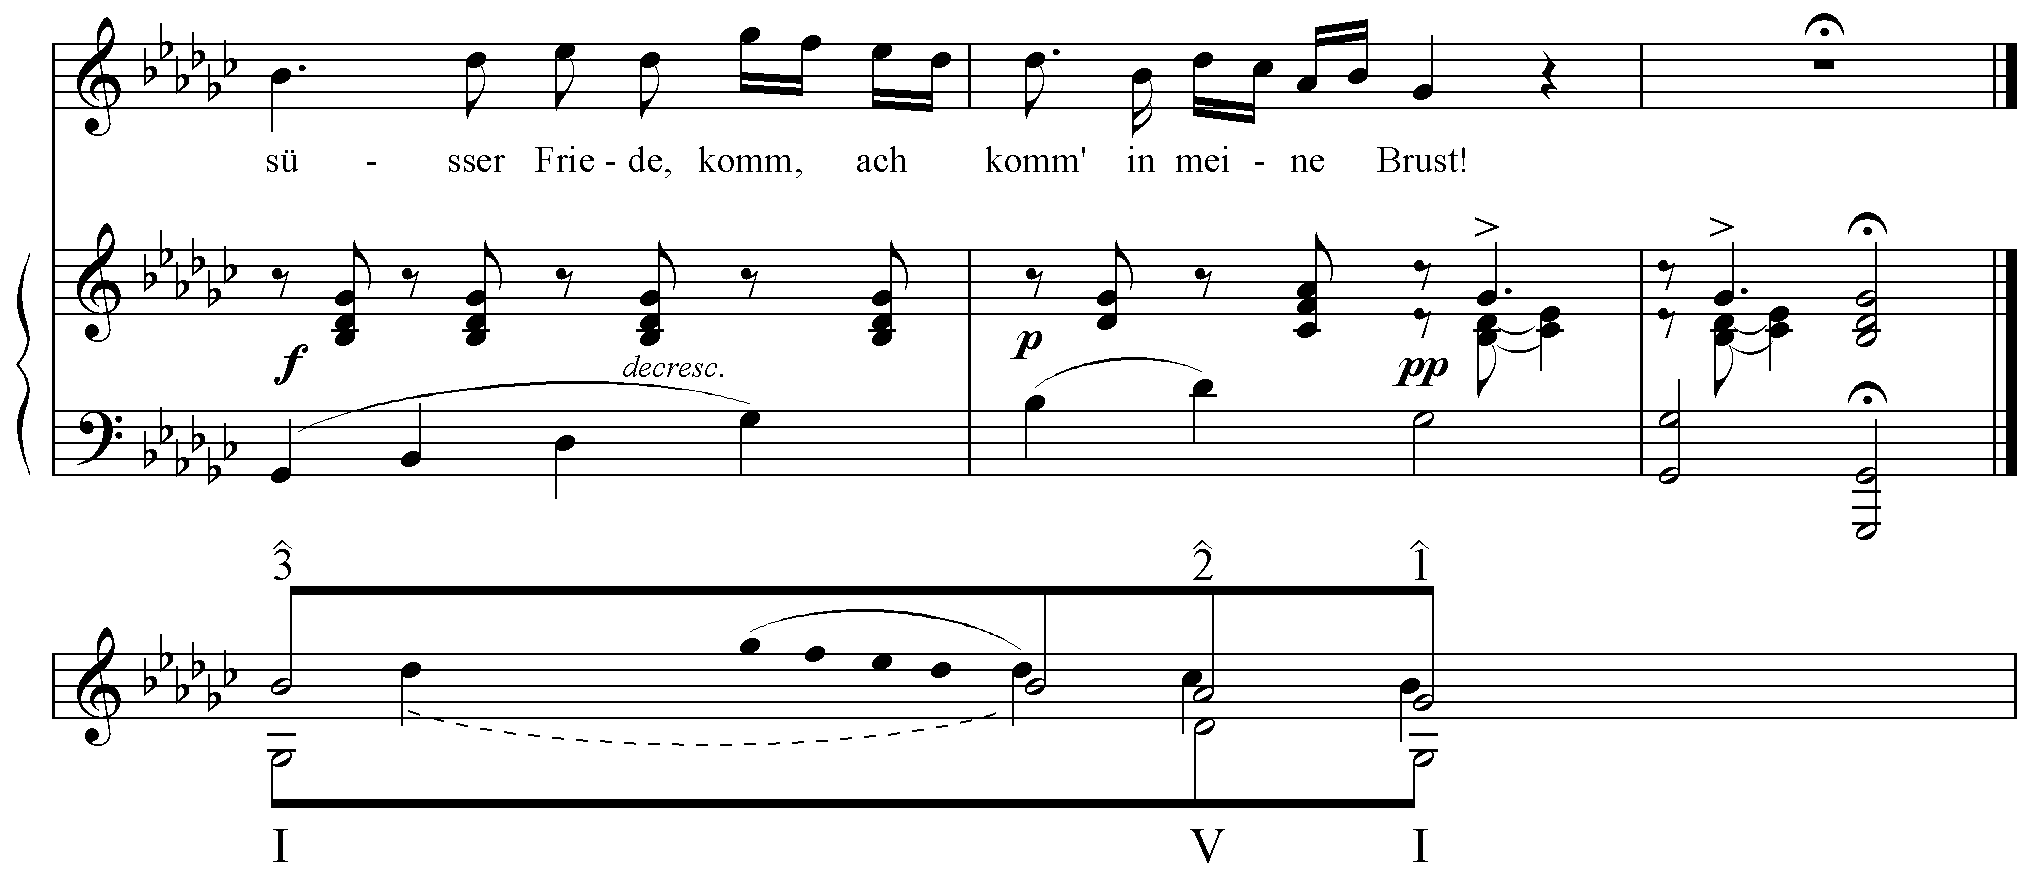
\includegraphics[clip,width=\columnwidth]{figures/schenkerian analysis/SchubertOp4no3.png}% 
\caption{\small{Small excerpt of \textit{Wandrers Nachtlied, Op. 4, D. 224} by Franz Schubert. We can see the passage's original score, the schenkerian unfolding of the melody, the chord degrees analysis, and the tonal function.}}
\label{fig:Wandrers Nachtlied, Op. 4, D. 224}
\end{figure}

%%%%%%%%%%%%%%%%%%%%%%%%%%%%%%%%%%%%%%%%%%%%

Schenkerian Analysis, developed by Austrian music theorist Heinrich Schenker, investigates the underlying structure of tonal music by focusing on the hierarchical relationships between pitches. This analytical approach is founded on the premise that all tonal music shares a fundamental structure known as "Ursatz" or "basic shape." The method identifies a piece's stepwise descending line (Urlinie) and bass arpeggiation (Bassbrechung), simplifying it to its essential elements and examining how different layers contribute to the overall structure. Central concepts in Schenkerian Analysis include prolongation levels, harmony, counterpoint, voice-leading, and Ursatz (fundamental structure). Despite criticism for reducing all tonal works to a limited number of background structures, Schenker highlights the significance of individual elaboration in determining a piece's identity and meaning.

While such analysis is designed for the symbolic domain, we argue that musical abstraction is also feasible in the audio time domain. In this section, we explore the application of Schenkerian Analysis principles to the Music Information Retrieval (MIR) domain by examining the foreground, middle-ground, and background levels of musical structure as follows:

\begin{itemize}
\item \textbf{Foreground}: The surface level of a musical composition, consisting of the notes, rhythms, and articulations directly perceived by the listener, representing the most detailed level of the musical structure.

\item \textbf{Middle-ground and mesostructures}: An intermediate level of analysis focusing on essential structural elements such as harmonic progressions, thematic materials, and voice-leading reductions that contribute to the overall composition. In the MIR domain, this level can also be understood as mesostructure. Mesostructures are intermediate levels of articulation between waveshapes' microstructure and musical forms' macrostructure. Examples of mesostructures include melody, arpeggios, syncopation, polyphonic grouping, and textural contrast. Mesostructures might have received limited attention in deep learning, as current models only focus on microstructures \cite{Mesostructures2023}.

\item \textbf{Background}: The most abstract level of musical structure, representing the fundamental core consisting of the \textit{Urlinie} and \textit{Bassbrechung}, which serves as the foundation for the entire composition.
\end{itemize}

By understanding and applying Schenkerian Analysis principles to the MIR domain, we can better understand the complex relationships between different levels of musical structure in the audio time domain, allowing for a more comprehensive analysis of tonal music.


%%%%%%%% PERCEPTION %%%%%%%%%%%%%

Kurt Koffka (1886-1941) was a German psychologist and a founding member of the Gestalt school of psychology, along with Max Wertheimer and Wolfgang Köhler. Gestalt psychology emerged as a reaction against the structuralist approach to psychology, emphasizing analyzing mental processes into their most basic elements. Instead, Gestalt psychologists sought to understand the principles underlying the organization and perception of complex forms and wholes.

Koffka's most significant contribution to the field was the development of the principles of Gestalt psychology and their application to perception. His 1935 book, ``Principles of Gestalt Psychology,'' remains a seminal work in the field \cite{Koffka2013PrinciplesPsychology}. In it, Koffka systematically describes the foundational concepts of Gestalt psychology and presents empirical evidence to support these ideas.

Applying the principles of Gestalt psychology to music can provide valuable insights into the cognitive processes underlying musical perception, organization, and interpretation. In music, just as in visual perception, the human mind seeks to identify patterns and structures to make sense of the auditory input. Several Gestalt principles can be applied to understanding musical perception, such as the law of Prägnanz, grouping principles, and holistic processing.

As with visual perception, the mind organizes musical information into the most straightforward and stable patterns. This principle can be observed in listeners' perceptions of harmony, melody, and rhythm. For example, Western tonal music is built upon hierarchical structures that allow the listener to make sense of complex musical information by organizing it coherently \cite{Lerdahl1985AMusic}.

In conclusion, applying the principles of Gestalt psychology to the study of music has led to a deeper understanding of the cognitive processes underlying musical perception and organization. This approach has influenced various areas of music research, including music theory, music cognition, and music therapy.

%%%%%%%%%%

Piaget's theory of cognitive development posits that children acquire knowledge from sensory and motor experiences in their early stages, from birth to around 18 months, during the \textit{sensorimotor stage} \cite{Huitt2003PiagetsDevelopment}. This stage sees the emergence of early representational thought through basic actions such as sucking, grasping, looking, and listening. As children progress through different developmental stages until adolescence and adulthood, their reasoning progressively moves toward abstract ideas and deductive logic. Schemas, higher-order cognitive structures hypothesized to underlie many aspects of human knowledge and skill, emerge during this process, which Piaget interprets through an equilibration mechanism that balances new information with old knowledge. This mechanism involves \textit{assimilation} and \textit{accommodation}, which entail taking in further information to fit pre-existing schemas and modifying existing schemas resulting from the latest information. In the context of learning, complex structures are based on simpler ones, and knowledge transfer occurs when dynamic systems capable of generalization are created. \cite{audioselfsupsurvey}

There are similarities between assimilation and accommodation in Piaget's theory of cognitive development and backpropagation in DL, both of which involve modifying existing structures based on new information. However, it should be noted that these processes' underlying mechanisms and contexts are entirely distinct. While assimilation and accommodation involve modifying mental structures to incorporate new information, backpropagation entails adjusting neural network weights to improve output predictions.

%%%%%%%%%%
